\subsection{(a)}

\includegraphics[width=13cm]{PCA_Eigen0.png}\\
\includegraphics[width=13cm]{PCA_Eigen1.png}\\
\includegraphics[width=13cm]{PCA_Eigen2.png}\\
\includegraphics[width=13cm]{PCA_Eigen3.png}\\
\includegraphics[width=13cm]{PCA_Eigen4.png}

\subsection{(b)}

\includegraphics[width=14cm]{Autoencoder_Error.png}\\
\includegraphics[width=14cm]{Denoising_Autoencoder_Error.png}

\subsection{(c)}

PCA mean squared error: $0.010710469688056315$.\\
\includegraphics[width=15cm]{PCA_Compare.png}\\
Autoencoder mean squared error: $0.012823789826138236$.\\
\includegraphics[width=15cm]{Autoencoder_Compare.png}\\
DenoisingAutoencoder mean squared error: $0.01361696472773301$.\\
\includegraphics[width=15cm]{Denoising_Autoencoder_Compare.png}

\subsection{(d)}

Architecture 1:\\
\tikzstyle{b} = [align=center, rectangle, draw, fill=white!20, text centered, rounded corners, thick]
\resizebox{15cm}{1.6cm}{
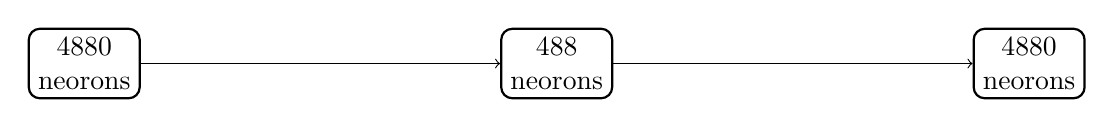
\begin{tikzpicture}[auto]
\node [b] (a) {4880\\neorons};
\node [b, right of=a, node distance=6cm] (b) {488\\neorons};
\node [b, right of=b, node distance=6cm] (c) {4880\\neorons};
\draw [->] (a) -- (b);
\draw [->] (b) -- (c);
\end{tikzpicture}
}
Mean squared error: $0.019768476466042514$.

Architecture 2:\\
\resizebox{15cm}{1.6cm}{
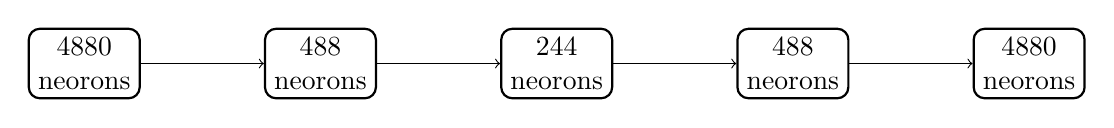
\begin{tikzpicture}[auto]
\node [b] (a) {4880\\neorons};
\node [b, right of=a, node distance=3cm] (b) {488\\neorons};
\node [b, right of=b, node distance=3cm] (c) {244\\neorons};
\node [b, right of=c, node distance=3cm] (d) {488\\neorons};
\node [b, right of=d, node distance=3cm] (e) {4880\\neorons};
\draw [->] (a) -- (b);
\draw [->] (b) -- (c);
\draw [->] (c) -- (d);
\draw [->] (d) -- (e);
\end{tikzpicture}
}
Mean squared error: $0.01361696472773301$.

Architecture 3:\\
\resizebox{15cm}{1.6cm}{
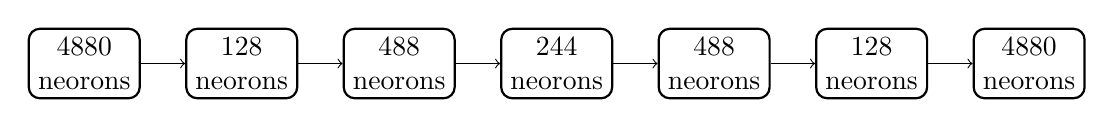
\begin{tikzpicture}[auto]
\node [b] (a) {4880\\neorons};
\node [b, right of=a, node distance=2cm] (b) {128\\neorons};
\node [b, right of=b, node distance=2cm] (c) {488\\neorons};
\node [b, right of=c, node distance=2cm] (d) {244\\neorons};
\node [b, right of=d, node distance=2cm] (e) {488\\neorons};
\node [b, right of=e, node distance=2cm] (f) {128\\neorons};
\node [b, right of=f, node distance=2cm] (g) {4880\\neorons};

\draw [->] (a) -- (b);
\draw [->] (b) -- (c);
\draw [->] (c) -- (d);
\draw [->] (d) -- (e);
\draw [->] (e) -- (f);
\draw [->] (f) -- (g);
\end{tikzpicture}
}
Mean squared error: $0.01518507843373457$\\
One can see that Architecture 2 has the best performance. The reason that Architecture 1 performs worse than Architecture 2 may be that it is not deep enough and therefore underfits the model. However, the deeper architecture doesn't imply the better performance. The reason that Architecture 3 performs worse than Architecture 2 may be that it is too deep and therefore overfits the model.

\subsection{(e)}

Adam:\\
\includegraphics[width=15cm]{Denoising_Autoencoder_Error.png}\\
Converged mean squared error: $0.01361696472773301$.\\
Accurracy: $0.9333333333333333$.\\\newpage
SGD:\\
\includegraphics[width=15cm]{sgd.png}\\
Mean squared error: $0.6925974951675007$.\\
Accurracy: $0.9$.\\\newpage
Adadelta:\\
\includegraphics[width=15cm]{adadelta.png}\\
Converged mean squared error: $0.08281828092189876$.\\
Accurracy: $0.7333333333333333$.\\
One can see that the error of SGD decreases slowly, and it's mean squared error after $500$ rounds is much more than the other two. Adam converges faster than the other two, and its performance (including error and accurracy) is also the best. Although SGD has high error, its accurracy is better than Adadelta. The reason may be that Adadelta overfits the model.
